\newpage
\section{Inbetriebnahme und Kalibration}

Da zum Zeitpunkt der Inbetriebnahme keine Topfmaschine von Leidolt Maschinenbau zur Verfügung stand, wurde ein Testaufbau erstellt. Dieser Testaufbau bildet den Topfkranz der Topfmaschine TC2 masstäblich ab. Auch soll die Rotation der Töpfe auf einfachste Weise funktionell umgesetzt werden. Wie im Pflichtenheft vorgesehen, wurde hierfür ein Kreisbogensegment durch vier Axiallager auf einer Grundplatte gelagert (siehe Abbildung \ref{fig:testaufbau}). Das Kreisbegensegment kann vier Töpfe aufnehmen. Dabei wurde der Radius des Bogensegments sowie der Winkel zwischen zwei Töpfen aus dem Datenblatt der TC2 entnommen (siehe Anhang). 

\begin{figure}[H]
	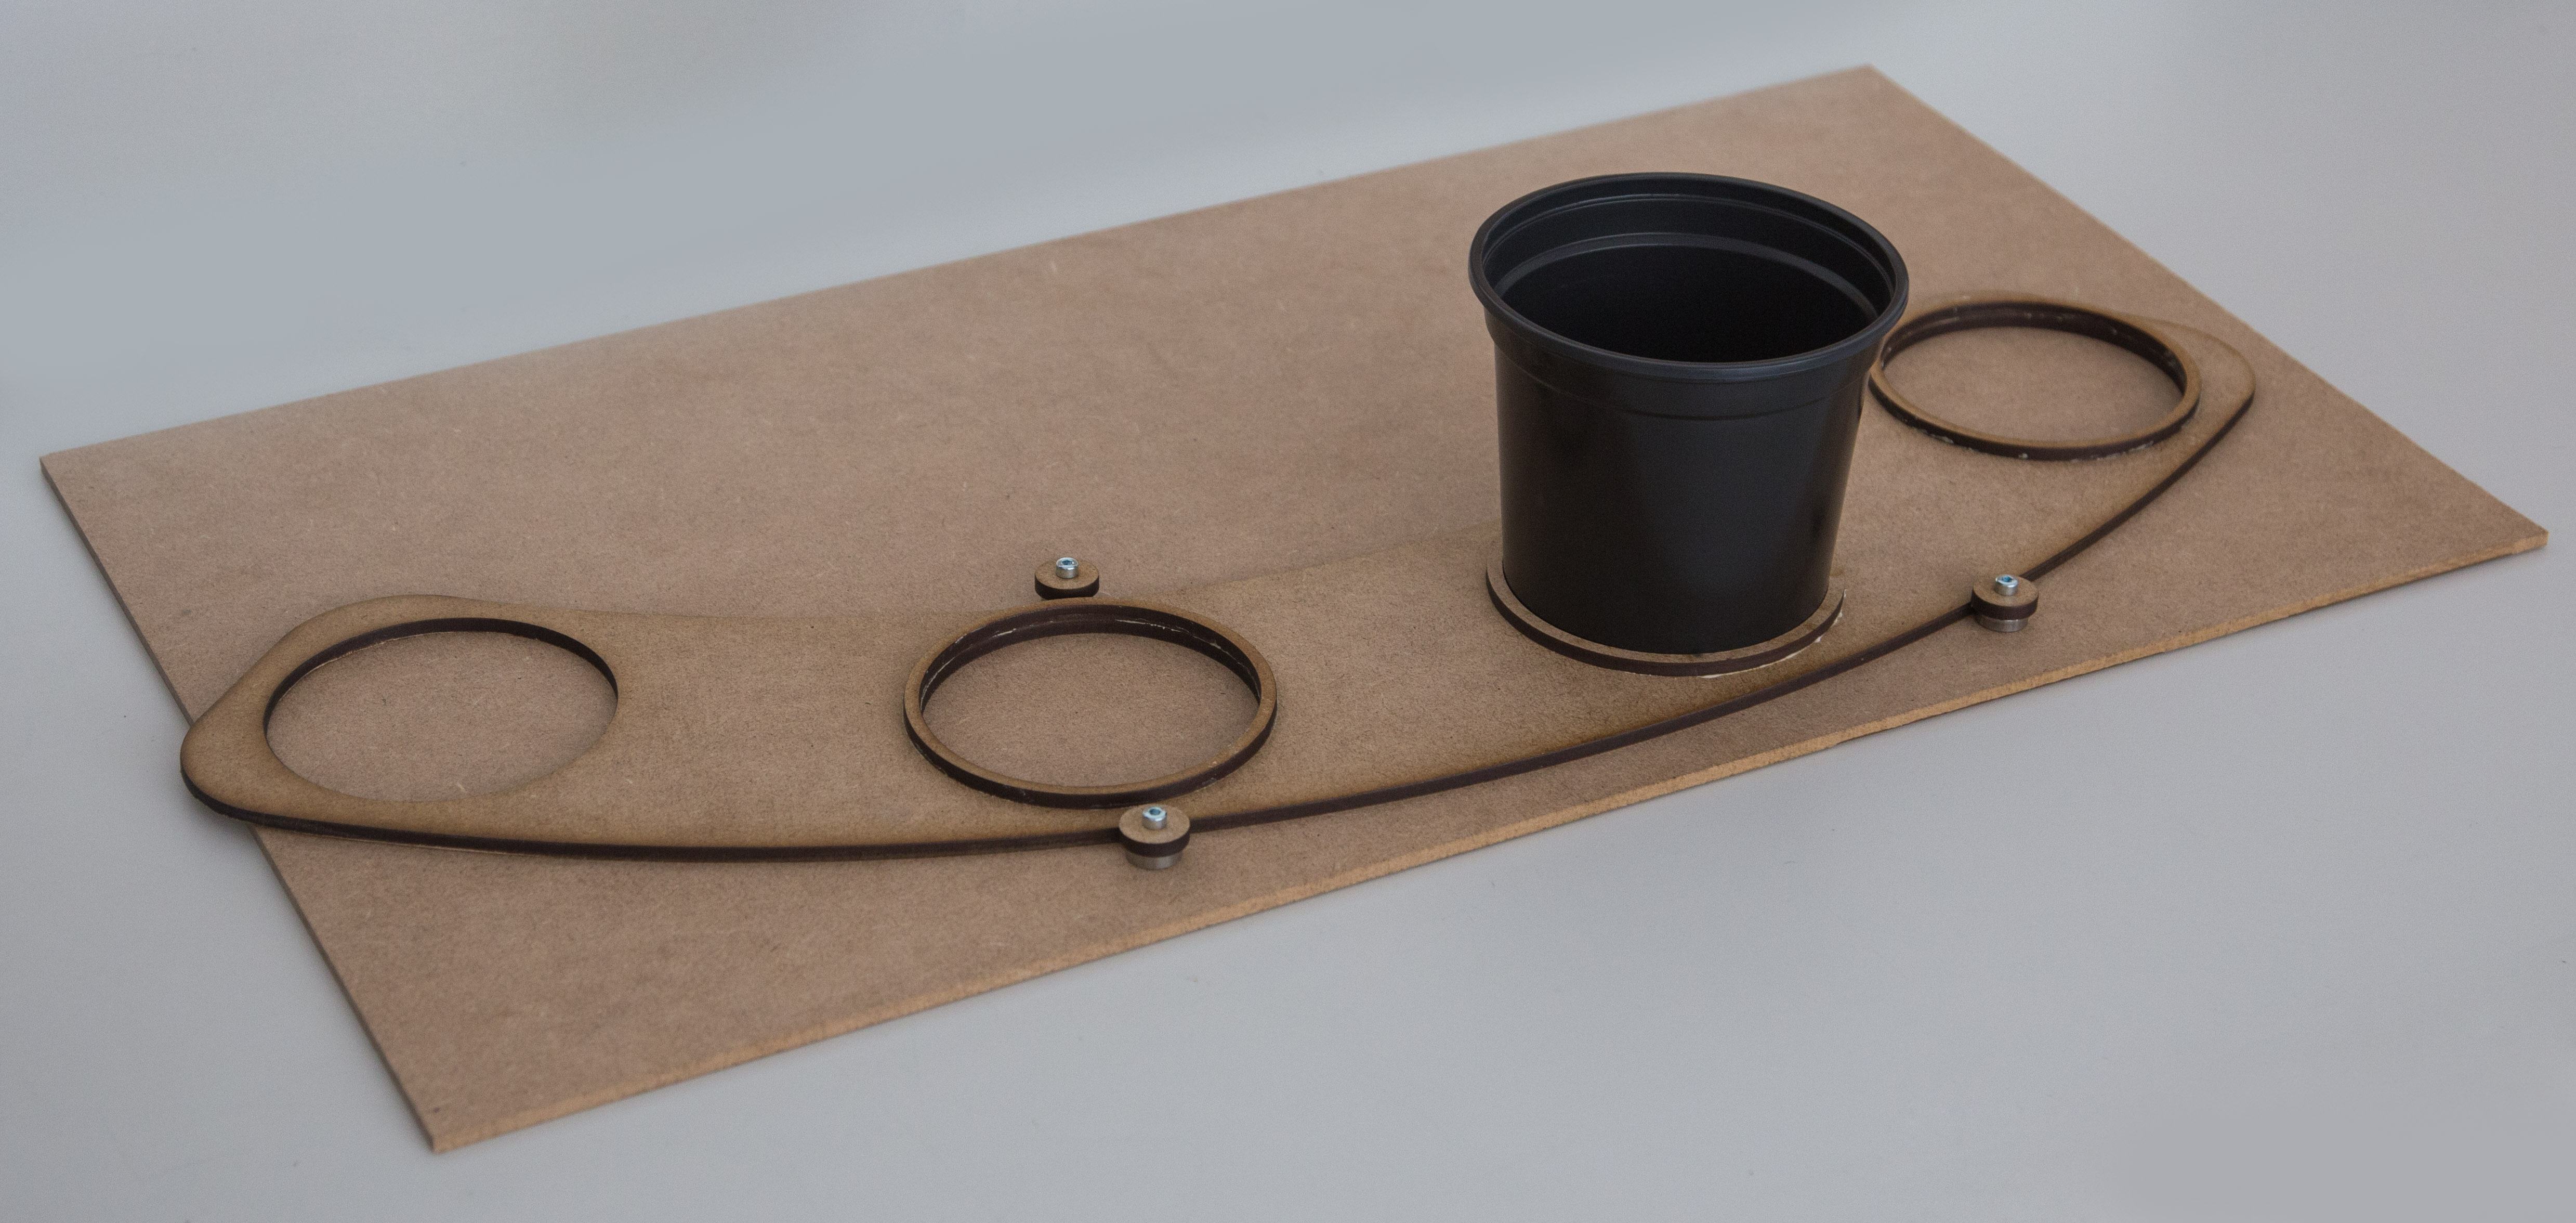
\includegraphics[width=1\textwidth]{Illustrationen/7-Inbetriebnahme_und_Kalibration/testaufbau.jpg}
	\caption{Testaufbau}
	\label{fig:testaufbau}
\end{figure}